\section{Introduction}
\label{sec:intro}

The advent of the FPGA revolutionized hardware design. It facilitated
rapid iteration and prototyping of a diverse array of new
architectures. The FPGA has provided these same benefits to the radio
space, spawning a new class of devices: software defined radios
(SDRs). The primary difference between traditional radios and a
software radio is the introduction of an FPGA to replace fixed
function components for low-level control and signal processing
logic. %as Figure~\ref{fig:radio_vs_sdr} shows.

Partridge predicts that by 2020, every commercial and military radio
will be an SDR system~\cite{patridge:SDR}. The military is well on its
way with the Joint Tactical Radio System
(JTRS~\cite{mitola2000sdr}). JTRS is the next generation voice
and data communication system for the U.S. military and is based on
the Software Communications Architecture (SCA~\cite{SCA}), an
open-architecture describing how software and hardware works
together. Commercial radios have slower to adopt the advantages of SDR
systems. GSM basestations are some of the first commercially available
SDR solutions~\cite{vocallo}. The rapid innovation and changes in
radio standards for cell phones places a big burden on the network
providers, as hardware has to be regularly upgraded. SDR basestations
alleviate this problem as simple firmware upgrades allow the radios to
adjust to the changes.

More general SDR hardware architectures offer high performance and are
optimized for
flexibility~\cite{soda,kuar,warp-platform,usrp:e100,usrp:n200,sora}. But
this has led to large, expensive, and power-hungry systems, ranging
from a few Watts to hundreds of Watts of power draw, and costing over
\$1,000 per radio. This development is contrary to the current
explosion of radio devices, which are small, portable, and usually
powered from batteries. If Partridge's prediction should become
reality, SDR systems must slim down, and start to explore the mobile
space.

\begin{comment}
Dutta et al. proposed one system architecture for putting the SDR
on a low-calorie diet~\cite{dutta-low-cal}. They identify four
requirements to achieve small, inexpensive, and low-power SDR systems:
\begin{description}
\item[\bf Radio Duty-Cycling] Many studies have shown that the radio
  is the major power draw in low-power wireless
  deployments~\cite{szewczyk04gdi,szlavecz06wise}. Prior work has
  shown the dependence of radio duty-cycling and key factors of a
  radio system~\cite{dutta07procrastinate}.
\item[\bf Low-Power FPGA] SDR systems typically distribute their
  functionality across many different components. Thus, it is not
  enough to optimize the radio frontend alone. Instead, we have to
  jointly optimize the radio frontend \emph{and} the backend
  processing usually performed in a FPGA or GPP
  in order to lower the total system power draw.
\item[\bf System Integration] SDR systems are built to be
  flexible. System developers expose this flexibility by implementing
  the different SDR components on different boards that get connected
  to each other over high-speed buses. This modularity inherently
  increases cost and size.
\item[\bf Measurement] The main goal of a mobile battery operated SDR
  system is low-power operation. Thus, such a system should integrate
  a comprehensive set of energy metering tools, exposing performance
  metrics for hardware and software.
\end{description}
\vspace{1em}

This work presents \sdr, the first instantiation of a recently
proposed SDR architecture~\cite{dutta-low-cal}. The goal of \sdr is to
explore the veracity of the claims made in the literature, to see how
close we can get with today's technologies, and to identify what open
problems and improvements are left to realize the vision of ubiquitous
software radios. But why can't we just make any of the already
existing platforms conform to those requirements? The answer lies in
their design, and the fact that they are intended for high-speed,
high-power applications. The point of low-power wireless protocols is
to reduce power draw. None of the existing SDR platforms achieve the
required power numbers.
\end{comment}

Mainstream (SRAM-based) FPGAs draw power in four distinct modes. 
In the powerup mode, the device (look-up tables, 
interconnect, I/O pads) must be configured, which requires initial 
charging of the distributed capacitances and causes a significant 
in-rush current to flow. Proper power sequencing can mitigate this 
problem, but cannot eliminate it completely. Then, the FPGA enters 
a configuration mode, which consists of shifting in a several megabits
long configuration bitstream. This stage also has a significant current 
drain and experiences non-trivial delay before the FPGA is ready for use. 
Finally, during normal operation, the SRAM-based FPGAs dissipate power in 
two different ways, during active operation and through static leakage. 
It is this static leakage in SRAM cells that dominates at low activity factors, and 
makes SRAM-based FPGA ill-suited to a low-power software radio platform.

Since static leakage dominates, traditional approaches to low-power 
operation become impossible. Frequency scaling, for example, addresses 
dynamic power so simply lowering or suspending the internal clocks 
cannot achieve truly low-power operational states on these devices. 
Voltage scaling, or power gating in the extreme, where the supply is
turned off, is not an effective solution either, and may create additional 
problems as well. First, by turning off power to the device, the memory 
contents will be lost. Second, the in-rush and reconfiguration currents 
are incurred on every subsequent powerup following a power down. 
These startup costs render any savings from the sleep mode
moot. Finally, latency incurred due to reconfiguration prevents fast or 
real-time wake-up techniques that are fundamental in low-power MAC protocols 
from being used. Therefore, duty cycling is limited to long sleep cycles and 
cases in which the discarding of the application state can be tolerated.

\begin{comment}
The design of \sdr addresses the power requirement by choosing an
flash-based FPGA and highly integrated components, thus reducing size,
cost, and power.  In particular, flash-based FPGAs can be duty-cycled,
whereas traditional SRAM-based ones cannot.  \sdr also relaxes some of
the flexibility that other SDR platforms provide, and integrates the
RF frontend, baseband processing, and application processor all on one
PCB board. Therefore, the RF frontend is fixed for a single radio
band. The advantage of this approach is the smaller component count as
no PCB interconnects are necessary. In addition, the physical size
reduces significantly, as no space has to be allocated for potential
future expansion boards or a modular interconnect. The higher
integration also reduces the manufacturing cost, resulting in a final
cost that is less than \$150.
\end{comment}


%Define low power radio space / requirements
%
%- Motivation: why do we need a low-power/mobile SDR
%- Should we introduce the concept of SDR here? A block-diagram comparing
%  regular radios to SDR might be useful.
%- Define requirements for low-power/mobile SDR (from HotNets paper?)
\begin{comment}
\begin{figure}[t]
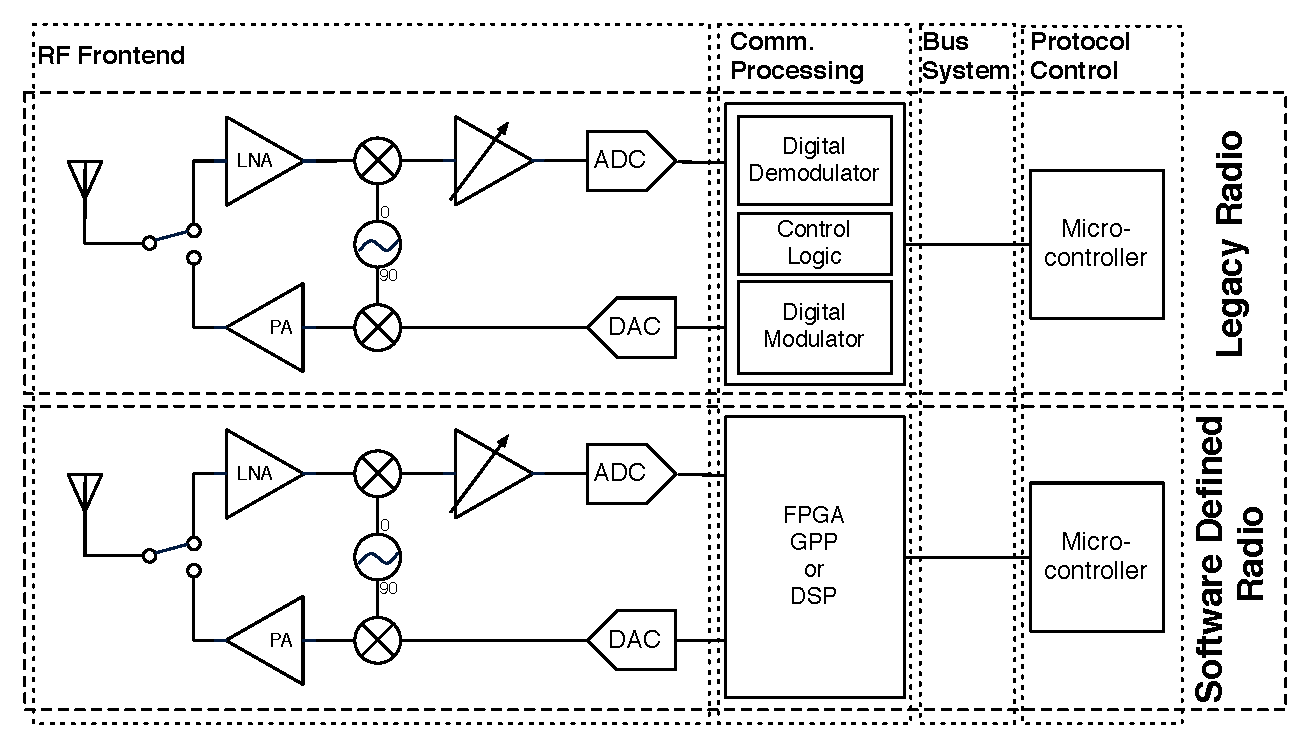
\includegraphics[width=0.98\columnwidth]{radio_vs_sdr}
\caption{Comparison of modern radio and a software defined radio. The main
difference is the fixed communication processing in a radio vs. the
reconfigurable processing possible in a SDR system.}
\label{fig:radio_vs_sdr}
\end{figure}
\end{comment}

\begin{table*}
\centering
\begin{threeparttable}
	\begin{tabular}{|l|c|c|c|c|c|c|c|} \hline
		\rowcolor[gray]{0}
		% header line
		\multicolumn{1}{|>{\columncolor[gray]{0}}c|}{\sc {\color{white} Platform}} &
		{\sc {\color{white} P$_{\text{Sleep}}$}} &
		{\sc {\color{white} P$_{\text{Active}}$}} &
		{\sc {\color{white} Size }}&
		{\sc {\color{white} Interconnect}}&
		{\sc {\color{white} Throughput}} &
		{\sc {\color{white} Price}} &
		% XXX: Usage -> adoption? Or some such metric is the idea behind this column
		{\sc {\color{white} Realization}}
		\\ \hline
		% SORA cost is totally estimated? No reference in the paper, but > PC cost..
		SORA {\small \cite{sora}}	 & -	& $>$100~W\tnote{c}	 & 36000~cm$^{3}$\tnote{c} & PCI-Express	& 16.7~Gb/s	& \$2000\tnote{c} & Research \\ \hline
		% KUAR power Pentium M min 5W, size COM Express 125 × 95 x (2 assumed) = 237.5, round 240, price: says "low cost" 3 times, but no price :(
		KUAR {\small \cite{kuar}}	 & -	& $>$5~W		 & 240~cm$^{3}$\tnote{f} &PCI-Express	& 2~Gb/s	& - & Research \\ \hline
		SODA {\small (180nm)~\cite{soda}} & -& \realtilde3~W & 26.6~mm$^{3}$\tnote{e}& DMA\tnote{a}	& 24~Mb/s\tnote{b} & -\tnote{d} & Simulated \\ \hline
		SODA {\small (90nm)~\cite{soda}} & -& \realtilde0.5~W & 6.7~mm$^{3}$\tnote{e}	& DMA\tnote{a}	& 24~Mb/s\tnote{b} & -\tnote{d} & Theoretical \\ \hline
		% WARP (numbers from energy wiki, where orig?), area 20 x 20 x >1, but we don't know it for sure so estimate conservative 2cm
		% Orig NRG num 10~15W, +30W / daughter card: 10~130W
		WARP~{\small \cite{warp-platform}} & -	& 10\realtilde130~W	 & 800~cm$^{3}$\tnote{f}	& Parallel MGTs\tnote{g}	& 24~Gb/s	& \$9750	 & Research \\ \hline
		%AirBlue Not really a platform
		% USRP 2, power 1.3-2.3A * 6V, area 22 x 16 x 5 cm
		% rate to/from host 50 MHz recv, 25 MHz xmit, 50/25 MSPS also
		% we'll go generous on the reported value
		USRP 2\tnote{c}~~{\small \cite{usrp:n200}}& -  & 7.9\realtilde13.8~W\tnote{c}	& 1760~cm$^{3}$\tnote{c} & Ethernet		& 1~Gb/s	& \$1700\tnote{c} & Commercial \\ \hline
		% E100, power 1.5-2.5A * 6V, area 22 x 16 x 5 cm
		% idle power is ~900mA * 6V = 5.5W
		% rate to/from host 4MHz, 4MSPS
% OMAP 3 GPMC Bus throughput: (we'll use best possible)
% http://e2e.ti.com/support/dsp/omap_applications_processors/f/42/t/35182.aspx#123019
		USRP E100~{\small \cite{usrp:e100}}& 5.5~W	& 9\realtilde15~W		 & 1760~cm$^{3}$		& OMAP 3 GPMC & 1.3~Gb/s	& \$1300	 & Commercial \\ \hline
		% uSDR, area 13 x 7 x 2
		\rowcolor[gray]{.9}
		\sdr	 & 0.32~W	& 1.4~W			 & 182~cm$^{3}$	& AMBA		& 1.4~Gb/s	& \$150\tnote{h}	 & Research \\ \hline
	\end{tabular}
	\begin{tablenotes}
		\small
		\item [a] Memory bus architecture not specified in~\cite{soda}.
		\item [b] Inferred minimum, may be faster.
		\item [c] Requires a companion PC. Not factored in power, portability, or cost for the USRP 1/2.
		\item [d] SODA is a custom chip that would likely have an extremely high die cost, but low per-unit cost.
		\item [e] Assumes $1mm$ thick.
		\item [f] Assumes $2cm$ thick.
		\item [g] ``Multi-Gigabit Transceiver'', an interconnect technology built into Xilinx FPGAs. Uses up to 8 parallel 3~Gb/s transceivers
		\item [h] Assumes 1,000 unit production run. See Table~\ref{tab:cost} for detailed breakdown.
	\end{tablenotes}
	\caption{A comparison of SDR platforms. The range in power comes from
boards whose power usage varies depending on the presence and type of daughter
card installed in the system. Where possible a measured idle / sleep power is
also shown.  For platforms that only list area we make reasonable assumptions
on height. \sdr is 10\% the cost of the next most expensive SDR platform, yet
provides parable speeds in the smallest non-IC package. It uses less power
than any realized hardware and nearly ties the previous best theoretical
hardware.}
	\label{tab:comparison}
\end{threeparttable}
\end{table*}
